\documentclass[aspectratio=1610, 12pt]{beamer}

\usepackage{fontspec}
\setmainfont{Latin Modern Roman}
\setsansfont{Latin Modern Sans}
\setmonofont{Latin Modern Mono}
\usefonttheme{serif}

\usepackage{xcolor}
\usepackage{amsmath, amssymb, mathtools}
\usepackage{booktabs, array, xcolor, graphicx}
\usepackage{tikz}
\usepackage{tcolorbox}
\tcbuselibrary{skins}

\definecolor{NavyBlue} {RGB}{0,   47,  95}
\definecolor{MedBlue}  {RGB}{0,  100, 180}
\definecolor{DarkRed}  {RGB}{158,  14,  14}
\definecolor{LightBg}  {RGB}{244, 246, 250}
\definecolor{MidGray}  {RGB}{208, 212, 220}
\definecolor{SlateGray}{RGB}{88,   96, 108}

\usetheme{default}
\setbeamertemplate{navigation symbols}{}
\setbeamertemplate{headline}{}
\setbeamercolor{background canvas}{bg=white}
\setbeamersize{text margin left=9mm, text margin right=9mm}

\setbeamercolor{frametitle}{fg=white, bg=NavyBlue}
\setbeamerfont{frametitle}{series=\bfseries, size=\large}
\setbeamertemplate{frametitle}{%
  \vspace{2pt}\hspace{4pt}\insertframetitle\vspace{2pt}%
}

\setbeamercolor{structure}       {fg=MedBlue}
\setbeamercolor{itemize item}    {fg=MedBlue}
\setbeamercolor{itemize subitem} {fg=SlateGray}
\setbeamertemplate{itemize item}    {\small$\bullet$}
\setbeamertemplate{itemize subitem} {\small$\circ$}

\newtcolorbox{defbox}[1][Definición]{%
  enhanced, colback=LightBg, colframe=NavyBlue,
  colbacktitle=NavyBlue, coltitle=white,
  fonttitle=\bfseries\footnotesize, title={#1},
  boxrule=0.9pt, arc=2pt,
  left=5pt, right=5pt, top=3pt, bottom=3pt,
  toptitle=2pt, bottomtitle=2pt}

\newtcolorbox{exbox}[1][Ejemplo]{%
  enhanced, colback=white, colframe=MedBlue,
  colbacktitle=MedBlue, coltitle=white,
  fonttitle=\bfseries\footnotesize, title={#1},
  boxrule=0.8pt, arc=2pt,
  left=5pt, right=5pt, top=3pt, bottom=3pt,
  toptitle=2pt, bottomtitle=2pt}

\newtcolorbox{alertbox}{%
  enhanced, colback=white, colframe=DarkRed,
  boxrule=0.8pt, arc=2pt,
  left=5pt, right=5pt, top=3pt, bottom=3pt}

\newcommand{\MT}{\textsc{mt}}
\newcommand{\blank}{\sqcup}

% --- DIAPOSITIVAS DE TRANSICIÓN DE SECCIÓN ---
\AtBeginSection[]{
  \begin{frame}[plain]
  \begin{tikzpicture}[remember picture, overlay]
    % Fondo azul marino
    \fill[NavyBlue] (current page.north west) rectangle (current page.south east);
    % Franja azul medio
    \fill[MedBlue] ([yshift=-31mm] current page.north west) rectangle ([yshift=-33mm] current page.north east);
    % Texto centrado
    \node[anchor=center] at (current page.center) {%
      \begin{minipage}{128mm}\centering
        {\color{white}\fontsize{24}{30}\selectfont\bfseries \insertsectionhead}
      \end{minipage}};
  \end{tikzpicture}
  \end{frame}
}

\begin{document}

% PORTADA
\begin{frame}[plain]
\begin{tikzpicture}[remember picture, overlay]

  \fill[NavyBlue]
    (current page.north west) rectangle (current page.south east);

  \node[anchor=north] at ([yshift=-5mm] current page.north) {%
    
\includegraphics[height=18mm]{unison.png}};

  \node[anchor=north, inner sep=0pt] at ([yshift=-25.5mm] current page.north) {%
    {\color{white!58}\fontsize{7.5}{9}\selectfont\itshape
      Universidad de Sonora \quad\textbar\quad Teoría de la Computación}};

  \fill[MedBlue]
    ([yshift=-31mm] current page.north west)
    rectangle
    ([yshift=-33mm] current page.north east);

  \node[anchor=center] at ([yshift=-2mm] current page.center) {%
    \begin{minipage}{128mm}\centering
      {\color{white}\fontsize{22}{28}\selectfont\bfseries
        Lenguajes Recursivos}\\[2.5mm]
      {\color{white}\fontsize{22}{28}\selectfont\bfseries
        y Problemas Decidibles}\\[4mm]
      {\color{white!52}\fontsize{8}{10}\selectfont Sección 8.2}
    \end{minipage}};

  \fill[NavyBlue!62!black]
    (current page.south west)
    rectangle ([yshift=17mm] current page.south east);

  \fill[MedBlue]
    ([yshift=17mm] current page.south west)
    rectangle ([yshift=17.8mm] current page.south east);

  \node[anchor=center] at ([yshift=8.5mm] current page.south) {%
    \begin{minipage}{148mm}\centering
      {\color{white!78}\fontsize{8.5}{11}\selectfont
        \textbf{Integrantes:}\enspace
        Gael Juan Valenzuela
        \enspace\textcolor{MedBlue!85}{$\cdot$}\enspace
        Angel Fernando Borquez Guerrero
        \enspace\textcolor{MedBlue!85}{$\cdot$}\enspace
        Owen Adiel Solis Zatarain
        \enspace\textcolor{MedBlue!85}{$\cdot$}\enspace
        Jorge Alan Ahumada Herrera\\[2.5mm]
        \color{white!45}2 de mayo de 2026}
    \end{minipage}};

\end{tikzpicture}
\end{frame}

\section{Máquinas de Turing como Algoritmos}

% SLIDE 2
\begin{frame}[t]{Máquinas de Turing como Algoritmos}
\vspace{4pt}
\begin{columns}[T]

  \begin{column}{0.50\textwidth}
    \begin{itemize}\setlength{\itemsep}{4pt}
      \item No toda \MT{}(Maquina de Turing) modela correctamente un algoritmo.
      \item \textbf{Ejemplo:} la \MT{} $M$ que imprime indefinidamente
        \[
          0\;1\;0\;1\;0\;1\;\cdots
        \]
        nunca alcanza una configuración de paro.
      \item No produce una respuesta definida
        $\;\Rightarrow\;$
        \textcolor{DarkRed}{\textbf{no es un algoritmo}}.
      \item Un buen modelo de algoritmo: \MT{} que \textbf{siempre termina}
        y produce una respuesta, desde cualquier configuración inicial.
    \end{itemize}
  \end{column}

  \begin{column}{0.46\textwidth}
    \begin{defbox}[Entrada y salida de una MT]
      \footnotesize
      Sea $M$ una \MT{} que siempre alcanza una configuración de paro.
      Dada la configuración inicial $(q_0,\,\underline{0}11101)$:
      \begin{itemize}\setlength{\itemsep}{3pt}
        \item[\textcolor{MedBlue}{$\bullet$}]
          $w = 011101$ es la \emph{entrada del algoritmo}.
        \item[\textcolor{MedBlue}{$\bullet$}]
          El cómputo llega a $(q,\;000001\blank)$,
          sin importar si $q \in F$ o no.
        \item[\textcolor{MedBlue}{$\bullet$}]
          Si $F = \emptyset$, la cinta es la \emph{salida del algoritmo}.
      \end{itemize}
      \vspace{3pt}
      Se escribe $M(w) = 000001$, es decir:
      \[
        (q_0,\,\underline{0}11101) \;\vdash^*\; (q,\,000001\blank)
      \]
    \end{defbox}
  \end{column}

\end{columns}
\end{frame}


% SLIDE 3
\begin{frame}[t]{Ejemplo 79 — MT para $w \pm 1$}
\vspace{4pt}
\begin{columns}[T]

  \begin{column}{0.46\textwidth}
    \begin{exbox}[Descripción de la máquina]
      \footnotesize
      La \MT{} $M$ recibe un número binario $w$ y calcula:
      \[
        M(w) =
        \begin{cases}
          w - 1 & \text{si } w \text{ es impar,}\\[2pt]
          w + 1 & \text{si } w \text{ es par.}
        \end{cases}
      \]
      \textbf{Observaciones:}
      \begin{itemize}\setlength{\itemsep}{2pt}
        \item $w$ par $\Leftrightarrow$ termina en $0$;\quad impar $\Leftrightarrow$ termina en $1$.
        \item Restar 1 al impar: reemplazar el último $1$ por $0$.
        \item Sumar 1 al par: reemplazar el último $0$ por $1$.
      \end{itemize}
      \vspace{2pt}
      Se tiene $F = \emptyset$.
    \end{exbox}
  \end{column}

  \begin{column}{0.50\textwidth}
    \small\textbf{Tabla de transiciones de $M$:}
    \vspace{4pt}

    {\footnotesize\renewcommand{\arraystretch}{1.45}%
    \begin{tabular}{>{$}c<{$} | >{$}c<{$} >{$}c<{$} >{$}c<{$}}
      \toprule
                       & 0                         & 1                         & \blank \\
      \midrule
      \rightarrow q_0  & (q_0,\,0,\,\rightarrow)  & (q_0,\,1,\,\rightarrow)  & (q_1,\,\blank,\,\leftarrow) \\
      q_1              & (q_2,\,1,\,\rightarrow)  & (q_2,\,0,\,\rightarrow)  & - \\
      q_2              & -                         & -                         & - \\
      \bottomrule
    \end{tabular}}

    \vspace{7pt}
    {\footnotesize
    \begin{itemize}\setlength{\itemsep}{3pt}
      \item[\textcolor{MedBlue}{$q_0$:}]
        Recorre la cinta a la derecha sin modificar nada.
      \item[\textcolor{MedBlue}{$q_1$:}]
        Modifica el último símbolo leído.
      \item[\textcolor{MedBlue}{$q_2$:}]
        Estado de paro; la salida queda en cinta.
    \end{itemize}}
  \end{column}

\end{columns}
\end{frame}


% SLIDE 4
\begin{frame}[t]{Ejemplo 79 — Cómputo de $17 - 1 = 16$}
\vspace{4pt}
\begin{columns}[T]

  \begin{column}{0.40\textwidth}
    \footnotesize
    $17 = 10001_{2}$ (impar)
    $\;\xrightarrow{M}\;$
    $10000_{2} = 16$

    \vspace{6pt}
    {\renewcommand{\arraystretch}{1.28}%
    \begin{tabular}{@{}r @{\hspace{8pt}} l@{}}
      \toprule
      \textbf{Estado} & \textbf{Cinta} \\
      \midrule
      inicio\; $q_0$ & $\underline{1}0001$ \\
      $q_0$          & $1\underline{0}001$ \\
      $q_0$          & $10\underline{0}01$ \\
      $q_0$          & $100\underline{0}1$ \\
      $q_0$          & $1000\underline{1}$ \\
      $q_0$          & $10001\underline{\blank}$ \\
      $q_1$          & $1000\underline{1}$ \\
      fin\; $q_2$    & $10000\underline{\blank}$ \\
      \bottomrule
    \end{tabular}}
  \end{column}

  \begin{column}{0.56\textwidth}
    \begin{defbox}[Análisis paso a paso]
      \footnotesize
      \begin{enumerate}\setlength{\itemsep}{4pt}
        \item[\textcolor{MedBlue}{1.}]
          $q_0$ avanza hacia la derecha
          \textbf{sin modificar} ningún símbolo.
        \item[\textcolor{MedBlue}{2.}]
          Al leer $\blank$: transita a $q_1$
          y \textbf{retrocede} una posición.
        \item[\textcolor{MedBlue}{3.}]
          $q_1$ lee el último dígito ($1$, impar)
          y lo \textbf{reemplaza por} $0$.
        \item[\textcolor{MedBlue}{4.}]
          $q_2$: configuración de paro.
          La salida en cinta es $10000 = 16$.
      \end{enumerate}
    \end{defbox}

    \vspace{6pt}
    \small\textbf{Notación compacta:}
    \[
      (q_0,\,\underline{1}0001)
      \;\vdash^*\;
      (q_2,\,10000\underline{\blank})
    \]
    \[
      M(10001) = 10000
    \]
  \end{column}

\end{columns}
\end{frame}

\section{Problemas de Decisión y Lenguajes Recursivos}
% SLIDE 5
\begin{frame}[t]{Problemas de Decisión con Máquinas de Turing}
\vspace{4pt}
\begin{columns}[T]

  \begin{column}{0.50\textwidth}
    Una \MT{} $M$ con $F \neq \emptyset$ que \textbf{no entra en ciclos infinitos}
    puede resolver un \textcolor{MedBlue}{\textbf{problema de decisión}}.

    \vspace{6pt}
    \textbf{Ejemplos de problemas de decisión:}
    \begin{itemize}\setlength{\itemsep}{4pt}
      \item ¿Es un número par?
      \item ¿Contiene un texto la palabra \textbf{sonora}?
      \item ¿Tiene un programa los paréntesis equilibrados?
      \item ¿Es una cadena un palíndromo?
    \end{itemize}

    \vspace{5pt}
    {\small\color{SlateGray}
      La entrada $w$ es, respectivamente, el número, el texto,
      el programa o la cadena.}
  \end{column}

  \begin{column}{0.46\textwidth}
    \begin{defbox}[Las dos posibilidades de $M(w)$]
      \footnotesize
      Dada una \MT{} $M$ y una entrada $w$:
      \vspace{4pt}
      \begin{itemize}\setlength{\itemsep}{4pt}
        \item[\textcolor{DarkRed}{$\bullet$}]
          \textbf{$M$ no se detiene:}
          \[ M(w) = \mathtt{loop} \]
        \item[\textcolor{MedBlue}{$\bullet$}]
          \textbf{$M$ para} y devuelve:
          \[
            M(w) =
            \begin{cases}
              \mathtt{true}  & \text{si } w \in L(M),\\[2pt]
              \mathtt{false} & \text{si } w \notin L(M).
            \end{cases}
          \]
      \end{itemize}
      \vspace{2pt}
      La salida depende de si el estado de paro
      es \textbf{de aceptación} o no.
    \end{defbox}
  \end{column}

\end{columns}
\end{frame}


% SLIDE 6
\begin{frame}[t]{Definición: Lenguaje Recursivo}
\vspace{4pt}

\begin{center}
\begin{tcolorbox}[%
  enhanced, width=0.78\textwidth,
  colback=LightBg, colframe=NavyBlue,
  colbacktitle=NavyBlue, coltitle=white,
  fonttitle=\bfseries\normalsize,
  title={Lenguaje Recursivo},
  boxrule=1.3pt, arc=3pt,
  left=8pt, right=8pt, top=5pt, bottom=5pt,
  toptitle=3pt, bottomtitle=3pt]
  \small
  Se dice que $L$ es un \emph{\textbf{lenguaje recursivo}} si existe una \MT{} $M$ tal que
  $L = L(M)$, y a partir de \textbf{cualquier configuración inicial} se llega a
  una \textbf{configuración de paro}.
\end{tcolorbox}
\end{center}

\vspace{5pt}
\begin{columns}[T]

  \begin{column}{0.50\textwidth}
    \begin{itemize}\setlength{\itemsep}{5pt}
      \item Son los lenguajes \textcolor{MedBlue}{\textbf{decidibles}}:
        existe un algoritmo que siempre responde
        si $w \in L$ o $w \notin L$.
      \item La \MT{} decisora \textbf{siempre para};
        nunca entra en $\mathtt{loop}$.
      \item Los lenguajes no recursivos corresponden a
        \textcolor{DarkRed}{\textbf{problemas indecidibles}}.
    \end{itemize}
  \end{column}

  \begin{column}{0.46\textwidth}
    \begin{alertbox}
      \small
      \textcolor{DarkRed}{\textbf{Pregunta clave:}}
      ¿Existen lenguajes que \emph{ninguna} \MT{} puede decidir?

      \vspace{4pt}
      La respuesta es \textbf{sí}. Eso estudia la \emph{indecidibilidad},
      que se formalizará en los siguientes slides.
    \end{alertbox}
  \end{column}

\end{columns}
\end{frame}

\section{El límite matemático: Indecidibilidad}
% SLIDE 7
\begin{frame}[t]{Indecidibilidad}
\vspace{2pt} % Margen superior reducido
\begin{columns}[T]

  \begin{column}{0.50\textwidth}
    \begin{defbox}[Problema indecidible]
      \small
      Un \emph{\textbf{problema indecidible}} es un problema de decisión
      caracterizado por un \textbf{lenguaje no recursivo}.

      \vspace{2pt} % Reducido
      Un problema que \textbf{no} es indecidible se llama \textbf{decidible}.
    \end{defbox}

    \vspace{3pt} % Espacio entre la caja y la lista reducido
    \small % <-- Tamaño de fuente más pequeño para la lista
    \begin{itemize}\setlength{\itemsep}{3pt} % Espacio entre viñetas reducido
      \item No existe ninguna \MT{} que, dada cualquier entrada,
        siempre responda \texttt{true} o \texttt{false}.
      \item Algunos lenguajes \textbf{no} pueden ser reconocidos
        por ningún algoritmo.
      \item La indecidibilidad no es una limitación tecnológica:
        es un \textcolor{DarkRed}{\textbf{límite matemático}} fundamental.
    \end{itemize}
  \end{column}

  \begin{column}{0.46\textwidth}
    \begin{defbox}[Jerarquía de lenguajes]
      \footnotesize
      \begin{center}
      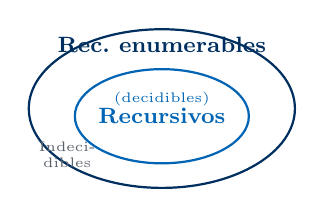
\begin{tikzpicture}[scale=0.65] 
        \draw[NavyBlue, thick] (0,0) ellipse (2.6cm and 1.55cm);
        \node[NavyBlue, font=\footnotesize\bfseries] at (0, 1.25) {Rec.\ enumerables};

        \draw[MedBlue, thick] (0,-0.15) ellipse (1.7cm and 0.92cm);
        \node[MedBlue, font=\footnotesize\bfseries] at (0,-0.15) {Recursivos};
        \node[MedBlue, font=\tiny] at (0,0.18) {(decidibles)};

        \node[SlateGray, font=\tiny, align=center] at (-1.85, -0.9)
          {Indeci-\\dibles};
      \end{tikzpicture}
      \end{center}
      \vspace{2pt}
      \scriptsize 
      Todo lenguaje recursivo es rec.\ enumerable,
      pero \textbf{no} al revés.
    \end{defbox}
  \end{column}

\end{columns}
\end{frame}


% SLIDE 8
\begin{frame}[t]{Ejemplo 80 — Ambigüedad en Gramáticas LC}
\vspace{4pt}
\begin{columns}[T]

  \begin{column}{0.50\textwidth}
    \begin{exbox}[Planteamiento]
      \footnotesize
      Se asigna a cada gramática libre de contexto (glc)
      una \textbf{codificación} $w$ sobre un alfabeto fijo $\Sigma$.

      \vspace{4pt}
      El lenguaje asociado al problema es:
      \[
        L_G \;=\; \{\,w \in \Sigma^* : w \text{ es una glc ambigua}\,\}
      \]

      \vspace{2pt}
      \textcolor{DarkRed}{\textbf{Resultado:}} $L_G$ \textbf{no es recursivo}.
    \end{exbox}

    \vspace{2pt}
    \begin{alertbox}
      \footnotesize % Reducido a footnotesize
      \textcolor{DarkRed}{\textbf{Conclusión:}}
      El problema de saber si una gramática libre de contexto
      es ambigua es \textbf{indecidible}.

      \vspace{3pt}
      No existe ningún algoritmo que, para toda glc $G$,
      determine en tiempo finito si $G$ es ambigua.
    \end{alertbox}
  \end{column}

  \begin{column}{0.46\textwidth}
    \begin{defbox}[¿Qué significa que $L_G$ no sea recursivo?]
      \scriptsize % Reducido a scriptsize
      \begin{enumerate}\setlength{\itemsep}{2pt} % Espaciado más ajustado
        \item[\textcolor{MedBlue}{1.}]
          Ninguna \MT{} $M$ puede decidir,
          para \textbf{toda} entrada $w$, si $w \in L_G$.
        \item[\textcolor{MedBlue}{2.}]
          Podría existir una \MT{} que reconozca
          algunas gramáticas ambiguas,
          pero \textbf{no todas}: entraría en loop
          para ciertos casos.
        \item[\textcolor{MedBlue}{3.}]
          El lenguaje $L_G$ pertenece a los
          \textbf{rec.\ enumerables no recursivos}.
      \end{enumerate}
    \end{defbox}

    \vspace{2pt}
    {\scriptsize\color{SlateGray}
      Este es uno de los problemas indecidibles más importantes
      para compiladores y procesamiento de lenguajes.}
  \end{column}

\end{columns}
\end{frame}

\section{La Tesis de Church-Turing}
% SLIDE 9 - Tesis de Church-Turing (I): Fundamentos y Equivalencias
\begin{frame}[t]{Tesis de Church-Turing (I): Fundamentos}
\vspace{4pt}
\begin{center}
\begin{tcolorbox}[%
  enhanced, width=0.85\textwidth,
  colback=LightBg, colframe=NavyBlue,
  colbacktitle=NavyBlue, coltitle=white,
  fonttitle=\bfseries\normalsize,
  title={La Tesis Central},
  boxrule=1.3pt, arc=3pt,
  left=8pt, right=8pt, top=5pt, bottom=5pt]
  \small
  «Todo algoritmo o procedimiento mecánico de cómputo puede ser llevado a cabo por una \textbf{Máquina de Turing}.»
\end{tcolorbox}
\end{center}

\vspace{5pt}
\begin{columns}[T]
  \begin{column}{0.50\textwidth}
    \begin{itemize}\small\setlength{\itemsep}{5pt}
      \item \textbf{Equivalencia histórica:} Alonzo Church ($\lambda$-cálculo) y Alan Turing (\MT) formularon modelos distintos que resultaron ser \textbf{idénticos} en poder.
      \item \textbf{Turing-Completitud:} Cualquier lenguaje de programación moderno es equivalente a una \MT.
    \end{itemize}
  \end{column}

  \begin{column}{0.46\textwidth}
    \begin{defbox}[¿Qué es computable?]
      \footnotesize
      La tesis define los límites de lo que es "calculable". Si una \MT{} no puede resolver un problema, se considera que dicho problema es \textbf{intrínsecamente no computable}.
    \end{defbox}
  \end{column}
\end{columns}
\end{frame}

% SLIDE 10 - Tesis de Church-Turing (II): Significado y Fronteras
\begin{frame}[t]{Tesis de Church-Turing (II): Trascendencia}
\vspace{4pt}
\begin{columns}[T]
  \begin{column}{0.50\textwidth}
    \begin{itemize}\small\setlength{\itemsep}{8pt}
      \item \textbf{¿Por qué es una Tesis?} No es un teorema matemático porque el concepto de "algoritmo" es una noción intuitiva, no una definición formal previa.
      \item \textbf{Evidencia empírica:} En casi un siglo, no se ha hallado ningún modelo físico o lógico que supere el poder de cómputo de la Máquina de Turing.
    \end{itemize}
  \end{column}

  \begin{column}{0.46\textwidth}
    \begin{alertbox}
      \small \textcolor{DarkRed}{\textbf{El límite del conocimiento:}}
      
      \vspace{4pt}
      Esta tesis marca la frontera final de la informática: establece que hay problemas que la lógica humana puede entender, pero que \textbf{ninguna máquina} podrá resolver jamás.
    \end{alertbox}

    \vspace{6pt}
    \begin{defbox}[Implicación en Decidibilidad]
      \scriptsize Un problema es \textbf{decidible} si y solo si existe una \MT{} que lo resuelva. La tesis asegura que esta definición es universal.
    \end{defbox}
  \end{column}
\end{columns}
\end{frame}



\section{Verificar que un lenguaje sea recursivo}

\begin{frame}[t]{Ejemplo final: $L_{012}$ es recursivo}
\vspace{4pt}
\begin{columns}[T]

  \begin{column}{0.50\textwidth}
    \begin{exbox}[Planteamiento]
      \footnotesize
      Consideremos el lenguaje:
      \[
        L_{012}=\{\,0^n1^n2^n : n>0\,\}
      \]

      \vspace{3pt}
      El ejercicio pide verificar que $L_{012}$ es
      \textbf{recursivo}.

      \vspace{4pt}
      Para demostrarlo, debemos describir una \MT{} que
      decida este lenguaje.
    \end{exbox}
  \end{column}

  \begin{column}{0.46\textwidth}
    \begin{defbox}[Objetivo]
      \footnotesize
      Queremos construir una \MT{} $M$ que:

      \begin{enumerate}\setlength{\itemsep}{3pt}
        \item acepte toda cadena de la forma $0^n1^n2^n$;

        \item rechace toda cadena que no tenga esa forma;

        \item siempre se detenga.
      \end{enumerate}

      \vspace{4pt}
      Si tal máquina existe, entonces $L_{012}$ es recursivo.
    \end{defbox}
  \end{column}

\end{columns}
\end{frame}


\begin{frame}[t]{Idea de la Máquina de Turing}
\vspace{4pt}
\begin{columns}[T]

  \begin{column}{0.50\textwidth}
    \begin{defbox}[Idea principal]
      \footnotesize
      Una cadena pertenece a $L_{012}$ si tiene la forma:
      \[
        0^n1^n2^n
      \]

      \vspace{2pt}
      Esto significa que por cada $0$ debe existir exactamente
      un $1$ y exactamente un $2$.

      \vspace{4pt}
      La \MT{} puede verificar esto marcando símbolos por grupos.
    \end{defbox}
  \end{column}

  \begin{column}{0.46\textwidth}
    \begin{exbox}[Marcas utilizadas]
      \footnotesize
      La máquina reemplaza los símbolos ya procesados por marcas:

      \[
        0 \to X,\qquad 1 \to Y,\qquad 2 \to Z
      \]

      \vspace{4pt}
      Donde:

      \begin{itemize}\setlength{\itemsep}{3pt}
        \item $X$ representa un $0$ ya usado;
        \item $Y$ representa un $1$ ya usado;
        \item $Z$ representa un $2$ ya usado.
      \end{itemize}
    \end{exbox}
  \end{column}

\end{columns}
\end{frame}


\begin{frame}[t]{Algoritmo de la Máquina de Turing}
\vspace{4pt}
\begin{columns}[T]

  \begin{column}{0.50\textwidth}
    \begin{defbox}[Primera revisión]
      \footnotesize
      Dada una cadena $w$, la máquina primero verifica que tenga
      la forma general:
      \[
        0^+1^+2^+
      \]

      \vspace{2pt}
      Es decir:

      \begin{itemize}\setlength{\itemsep}{3pt}
        \item primero deben aparecer únicamente ceros;
        \item después únicamente unos;
        \item al final únicamente doses.
      \end{itemize}

      \vspace{4pt}
      Si aparece un símbolo fuera de orden, la máquina rechaza.
    \end{defbox}
  \end{column}

  \begin{column}{0.46\textwidth}
    \begin{alertbox}
      \small
      \textcolor{DarkRed}{\textbf{Ejemplos de orden incorrecto:}}

      \vspace{4pt}
      \[
        010122,\qquad 001212,\qquad 120
      \]

      \vspace{4pt}
      Estas cadenas se rechazan porque no respetan el orden
      $0^+1^+2^+$.
    \end{alertbox}
  \end{column}

\end{columns}
\end{frame}


\begin{frame}[t]{Marcado de símbolos}
\vspace{4pt}
\begin{columns}[T]

  \begin{column}{0.50\textwidth}
    \begin{defbox}[Proceso repetitivo]
      \footnotesize
      Después de verificar el orden, la máquina regresa al inicio
      de la cinta y repite el siguiente proceso:

      \begin{enumerate}\setlength{\itemsep}{4pt}
        \item busca el primer $0$ sin marcar;

        \item si lo encuentra, lo cambia por $X$;

        \item busca hacia la derecha el primer $1$ sin marcar;

        \item si lo encuentra, lo cambia por $Y$;

        \item busca hacia la derecha el primer $2$ sin marcar;

        \item si lo encuentra, lo cambia por $Z$.
      \end{enumerate}
    \end{defbox}
  \end{column}

  \begin{column}{0.46\textwidth}
    \begin{exbox}[Interpretación]
      \footnotesize
      Cada vuelta del proceso marca un grupo completo:

      \[
        0,\;1,\;2
      \]

      \vspace{4pt}
      Es decir, la máquina empareja un $0$ con un $1$ y con un $2$.

      \vspace{4pt}
      Si en algún momento encuentra un $0$, pero ya no hay un $1$
      o un $2$ disponible, entonces la cadena no tiene la misma
      cantidad de símbolos y se rechaza.
    \end{exbox}
  \end{column}

\end{columns}
\end{frame}


\begin{frame}[t]{Condición final de aceptación}
\vspace{4pt}
\begin{columns}[T]

  \begin{column}{0.50\textwidth}
    \begin{defbox}[Cuando ya no hay ceros]
      \footnotesize
      El proceso se repite hasta que ya no exista ningún $0$
      sin marcar.

      \vspace{4pt}
      En ese momento, la máquina realiza una última revisión
      de la cinta.

      \vspace{4pt}
      Si todos los símbolos fueron marcados, entonces la cinta
      solo contiene símbolos de la forma:
      \[
        X^nY^nZ^n
      \]
    \end{defbox}
  \end{column}

  \begin{column}{0.46\textwidth}
    \begin{alertbox}
      \small
      \textcolor{DarkRed}{\textbf{Criterio final:}}

      \vspace{4pt}
      La máquina acepta si solo quedan símbolos marcados:

      \[
        X,\quad Y,\quad Z
      \]

      \vspace{4pt}
      La máquina rechaza si queda algún símbolo sin marcar:

      \[
        0,\quad 1,\quad 2
      \]

      \vspace{4pt}
      Esto asegura que había la misma cantidad de $0$, $1$ y $2$.
    \end{alertbox}
  \end{column}

\end{columns}
\end{frame}


\begin{frame}[t]{Ejemplo de aceptación}
\vspace{4pt}
\begin{columns}[T]

  \begin{column}{0.50\textwidth}
    \begin{exbox}[Entrada]
      \footnotesize
      Consideremos la cadena:
      \[
        000111222
      \]

      \vspace{4pt}
      La máquina marca un $0$, un $1$ y un $2$ en cada repetición.

      \vspace{4pt}
      Primera repetición:
      \[
        000111222
        \;\Rightarrow\;
        X00Y11Z22
      \]

      Segunda repetición:
      \[
        X00Y11Z22
        \;\Rightarrow\;
        XX0YY1ZZ2
      \]
    \end{exbox}
  \end{column}

  \begin{column}{0.46\textwidth}
    \begin{defbox}[Resultado]
      \footnotesize
      Tercera repetición:
      \[
        XX0YY1ZZ2
        \;\Rightarrow\;
        XXXYYYZZZ
      \]

      \vspace{4pt}
      Ya no quedan ceros sin marcar.

      \vspace{4pt}
      Además, tampoco quedan unos ni doses sin marcar.

      \vspace{4pt}
      Por lo tanto, la máquina acepta:
      \[
        000111222 \in L_{012}
      \]
    \end{defbox}
  \end{column}

\end{columns}
\end{frame}


\begin{frame}[t]{Ejemplo de rechazo}
\vspace{4pt}
\begin{columns}[T]

  \begin{column}{0.50\textwidth}
    \begin{exbox}[Entrada]
      \footnotesize
      Consideremos la cadena:
      \[
        0011222
      \]

      \vspace{4pt}
      La máquina puede marcar dos grupos completos:

      \[
        0011222
        \;\Rightarrow\;
        X0Y1Z22
      \]

      \[
        X0Y1Z22
        \;\Rightarrow\;
        XXYYZZ2
      \]
    \end{exbox}
  \end{column}

  \begin{column}{0.46\textwidth}
    \begin{alertbox}
      \small
      \textcolor{DarkRed}{\textbf{Resultado:}}

      \vspace{4pt}
      Ya no quedan ceros sin marcar.

      \vspace{4pt}
      Sin embargo, todavía queda un $2$ sin marcar:

      \[
        XXYYZZ2
      \]

      \vspace{4pt}
      Esto significa que no había la misma cantidad de $0$, $1$ y $2$.

      \vspace{4pt}
      Por lo tanto:
      \[
        0011222 \notin L_{012}
      \]
    \end{alertbox}
  \end{column}

\end{columns}
\end{frame}



% SLIDE 11 — CIERRE
\begin{frame}[plain]
\begin{tikzpicture}[remember picture, overlay]

  \fill[NavyBlue]
    (current page.north west) rectangle (current page.south east);

  \fill[MedBlue]
    ([yshift=-31mm] current page.north west)
    rectangle
    ([yshift=-33mm] current page.north east);

  \node[anchor=center] at ([yshift=5mm] current page.center) {%
    \begin{minipage}{118mm}\centering
      {\color{white}\fontsize{13}{18}\selectfont\bfseries Resumen}\\[5mm]
      {\color{white!80}\fontsize{10.5}{15}\selectfont
        \begin{tabular}{@{}>{\color{MedBlue}\bfseries}r @{\enspace}
                           >{\color{white!85}}l@{}}
          Lenguaje recursivo   & MT que \emph{siempre} para y decide $w \in L$ o no. \\[3pt]
          Problema decidible   & Caracterizado por un lenguaje recursivo. \\[3pt]
          Problema indecidible & Lenguaje no recursivo; ningún algoritmo lo resuelve. \\[3pt]
          Tesis Church-Turing  & Todo algoritmo es simulable por una MT. \\[3pt]
          Ejemplo indecidible  & Ambigüedad de gramáticas libres de contexto.
        \end{tabular}
      }
    \end{minipage}};

  \fill[NavyBlue!62!black]
    (current page.south west)
    rectangle ([yshift=17mm] current page.south east);

  \fill[MedBlue]
    ([yshift=17mm] current page.south west)
    rectangle ([yshift=17.8mm] current page.south east);

  \node[anchor=center] at ([yshift=8.5mm] current page.south) {%
    {\color{white!60}\fontsize{9}{12}\selectfont
      Universidad de Sonora \enspace\textcolor{MedBlue!85}{$\cdot$}\enspace
      Teoría de la Computación \enspace\textcolor{MedBlue!85}{$\cdot$}\enspace
      Sección 8.2}};

\end{tikzpicture}
\end{frame}








\end{document}
